% !TEX encoding = UTF-8

\documentclass[fleqn]{IEEEtran}
\usepackage[T1]{fontenc}
\usepackage[utf8]{inputenc}
\usepackage[italian, english]{babel}
\usepackage{graphicx}
\usepackage{booktabs}
\usepackage{listings}
\usepackage{amsmath}


\title
{
Parallel CRC Algorithm\\and Implementation with CUDA
}
\author{Mirco De Marchi - VR445319 \and Luigi Capogrosso - VR445456}

\begin{document}


\maketitle


\begin{abstract}
\textit{Cyclic redundancy checks (CRCs)} form a powerful class of codes suited especially 
for the detection of burst errors in data storage and communication 
applications. The use of cyclic redundancy codes, referred to more briefly 
in this document as check words, is one of the most weel known error checking mechanism. It is 
customarily placed at the end of a data block, occupying one or more bytes of the 
transmitted message. In this paper, we present a \textit{Parallel Cyclic 
Redundancy Check (PCRC)} algorithm improved with CUDA. Our approach is to 
systematically decompose the original input message into a set of subsequences 
based on the \textit{Galois field} theory.
\end{abstract}


\section{State of the art}
Devices such as computers, routers, networking equipment, and components 
that communicate information internally and/or with other devices. For 
example, computers might communicate across a local area network (LAN) using 
Ethernet protocol, or application-specific integrated circuits (ASICs) may 
communicate with each other over a single or parallel bit bus. \textbf{It is 
important for these devices to reliably communicate and detect errors in 
their communication}.

One common technique for detecting transmission errors is a technique known as 
\textbf{cyclic redundancy check (CRC)}. A CRC allows errors detection using 
only a small number of redundant bits typically sent along with the 
communicated information. For example, a 32-bit CRC gives strong protection 
against burst bits errors in messages that are thousands bits long. 

The fundamental principle upon which CRC is based can be expressed equivalently 
in one of three ways.

\begin{enumerate}
	\item CRC can be described in terms of binary numbers division;
	\item It can be performed utilizing a polynomials division;
	\item The utility in implementing CRCs is often realized by designing special 
	check circuits in which Exclusive Or (XOR) and other elementary binary 
	operands generate partial results that can be used in CRC algorithm;
\end{enumerate} 

CRCs are specifically designed to protect against common types of errors 
on communication channels, where they can provide quick and reasonable 
assurance of the integrity of the messages delivered. However, CRCs are
not suitable for protecting against intentional alteration of data.


\section{Introduction}
Modern day technology permits a large amounts of data tranfer between 
computer or communication systems. During transmission these bits may become 
altered, thereby creating an error. In order for one computer system to detect 
when data sent by another computer system has an error, certain status 
information is often transmitted along with the data. This status information 
may include parity (even or odd), longitudinal redundancy check character, 
or cyclic redundancy check code.

CRCs are based on the theory of \textbf{systematic cyclic codes}, which encode 
messages by adding a fixed-length check value. Cyclic codes are not only simple
to implement but \textbf{have the benefit of being particularly well suited 
for the detection of burst errors}: contiguous sequences of erroneous data 
symbols in messages.

Specification of a CRC code requires definition so-called 
\textbf{generator polynomial}. For the purposes of constructing polynomial codes, 
we identify a string of $n$ symbols $a_{n-1},\dots{},a_{0}$ with the polynomial:
\[
   a_{n-1}x^{n-1}+\dots{}+a_{1}x+a_{0}
\]

This polynomial becomes the \textbf{divisor} in a 
\textbf{polynomial long division}, which takes the message as the 
\textbf{divident}, the \textbf{quotient} is discarded and the 
\textbf{remainder} becomes the result. The important is that \textbf{the 
polynomial coefficients are calculated according to the arithmetic of a finite 
field}, so the addition operation can always be performed bitwise-parallel 
(there is no carry between digits). A finite field is a set on which the 
operations of multiplication, addition, subtraction and division are 
defined and satisfy certain basic rules.

A CRC is called an $N$-bit CRC when its check value is $N$ bits long. The 
simplest error-detection system, the parity bit, is in fact a 1-bit CRC: 
it uses the generator polynomial $x + 1$ (two terms), and has the name CRC-1.

A CRC-enabled device calculates a short, fixed-length binary sequence, known 
as CRC, that will be appended to the end of message sent. The receiving device 
recalcutes the CRC code over the received message payload and If the CRC 
values do not match, then the mesage contains a 
data error. The device may take corrective action, such as rereading the block 
or requesting that it be sent again. Otherwise, the data is assumed to 
be error-free.

The common hardware solution is the “Linear Feedback Shift Register” (LFSR), 
which is a simple bitwise architecture for both encoding and deconding the 
message. This approach typically calculates the CRC for a $N$-bit message in 
$N$ clock cycles. This approach is not efficient at high bit rates.


\section{Backgorund}
The CRC see the message $A$ of length $n$ as a polynomial $A(x)$ of degree $n-1$
in which every bit of message is the coefficient of the respective monomial:
\[
   A=[a_{n-1},a_{n-2},\dots{},a_{2},a_{1},a_{0}]
\]
\[
   A(x)=a_{n-1}x^{n-1}+a_{n-2}x^{n-2}+\dots{}+a_{2}x^{2}+a_{1}x+a_{0}
\]
For example, the input data \verb|Ox25=0010 0101| is taken as:
\[
   A(x)=0x^{7}+0x^{6}+1x^{5}+0x^{4}+0x^{3}+1x^{2}+0x^{1}+1x^{0}
\]

Then for the CRC computation is used a polynomial generator $G(x)$ that is 
polynomial of degree $m$. The major index coefficient is always $1$, in this 
way the polynomial generator guarantees to always be of $m$ degree. 

In a reverse way the than the message $A$, the polynomial generator can be 
represented as a sequence of bit $G$ of size $m+1$ with the most significant bit 
always to $1$. This the reason why you will always find the value representation 
of the polynomial generator $G$ of size $m$, because the bit $1$ to the left is 
implicit.
\[
   G=[g_{m},g_{m-1},\dots{},g_{1},g_{0}] 
\]
\[
   G=g_{m}x^{m}+g_{m-1}x^{m-1}+\dots{}+g_{1}x+g_{0}
\]
For example, Ethernet uses the following 32-bit polynomial value:
\begin{gather*}
   G(x)=1+x+x^{2}+x^{4}+x^{5}+x^{7}+x^{8}+x^{10}+x^{11} \\
   +x^{12}+x^{16}+x^{22}+x^{23}+x^{26}+x^{32}
\end{gather*}

The \textbf{value of the polynomial generator} has a 
\textbf{great impact on its error detection} capabilities, its design is 
non-trivial and requires serious math knowledge.

\textbf{The CRC detection code is the result of the reminder after dividing the 
origninal message $A$ concatenated with $m$ zero bits by a polynomial generator
in binary modulo 2 arithmetic}.

In the polynomial version this definition of CRC is equivalent to:
\[
   CRC[A(x)]=A(x)x^{m}mod2(G(x))
\]

The binary modulo 2 arithmetic makes every operation between bits indipendent
between each other. This means that \textbf{the carry bit can be completely 
forgotten}. In practice the arithmetic operations are identical but the carryover 
is ignored. In particular the binary modulo 2 reminder of the division always 
generates a result that is a degree less of the degree of the divisor. Therefore
the CRC result will always be a polynomial of degree $m-1$ that can be viewed as
a binary code of size $m$. In fact:
\[
   CRC[A(x)]=A(x)x^{m}mod2(G(x))
\]
is equal to:
\[
   degree(CRC[A(x)])=m-1
\]

This beacuse the main difference between different CRC code is the length $m$ of
the code generated. The most important CRC Implementations are \textbf{CRC8}, 
\textbf{CRC16}, \textbf{CRC32} and \textbf{CRC64}. The longer the length of the 
CRC code, the more likely bit errors shall be detected. 
In general if a network protocol provides very long message should be used a 
longer CRC as CRC32 or CRC64, if a network exchanges short message can be used 
shorter CRC error detection code as CRC8 or CRC16.

Then there are different parametrization of the CRC:
\begin{itemize}
   \item \textbf{Polynomial generator}: normal, reversed (from the least 
   significant bit to the most), reciprocal (reversed but respect the polynomial 
   coefficients), reversed and reciprocal in combination and the Koopman
   representation (discarding the least significant bit);

   \item \textbf{Initial value of the CRC}: in most algorithms is $0$, in some 
   cases is set with all bit to $1$, but in general could be any value;

   \item \textbf{Input reflected}: each input byte can be used in reverse order 
   before being used in the calculation;

   \item \textbf{Output reflected}: the result can be returned in reverse order 
   over the whole CRC value;

   \item \textbf{Final XOR value}: is value xored to the final CRC value before 
   being returned and, in case, after the output reflected step.
\end{itemize}


\section{Lemmas}
Before we present our parallel CRC algorithm, we need the following lemma, 
which gives the well-known congruence properties for polynomial division.

\begin{small}
\begin{gather}
   (A(x)+B(x))modG(x)=A(x)modG(x)+B(x)modG(x) \\
   \begin{split}
   A(x)B(x)modG(x)= & ((A(x)modG(x))(B(x)modG(x))) \\ & modG(x)
   \end{split}
\end{gather}
\end{small}

There is a system of arithmetic known as \textbf{Galois field arithmetic}. 
A Galois field is an example of algebraic field, which has a set of elements 
called \textbf{numbers or field elements}, and a definition of two operations 
called \textbf{addition and multiplication }such that the formal properties 
satisfied by the real arithmetic system (e.g. commutativity, associativity, and
distributivity) are satisfied. 

For each positive integer $M$, there is a Galois field called $GF(2^{M})$ that 
has $2^{M}$ elements in it. The set of elements of $GF(2^{M})$ can be
represented as the set of $M$-bit binary numbers in the range from $0$ to 
$2^{M}-1$. The addition over Galois Field $GF(2^{M})$ is defined as bit-by-bit 
modulo-2 addition which is equivalent to exclusive-or (i.e., XOR) operation.

\textbf{In practice, all commonly used CRCs employ the Galois field of two 
elements}, $GF(2)$. The two elements are usually called 0 and 1, 
comfortably matching computer architecture. Multiplication of two elements $a$ 
and $b$ in $GF(2^{M})$ will produce an element $c=ab$ by polynomial 
multiplication modulo the irreducible polynomial G(x):
\[
   C(x)=A(x)B(x)modG(x)
\]
where $A(x)$, $B(x)$ and $C(x)$ is the polynomial form of $a$, $b$, and $c$, 
respectively.


\section{CRC algorithms}
Common CRC algorithms are bitwise and bytewise. 

\textbf{In the bitwise CRC algorithm, 1 input bit is processed at a time as 
the name indicates, using long division}. 

First we append $M$ zeros ($M$ is the number of bits in CRC) to the original 
$N$-bit message to the least significant bit (LSB) and define the appended 
message as a running message. 

Second, check the most significant bit (MSB) of the running message. 

If the MSB of the running message is $1$, subtract the generator polynomial 
from the $M$ most significant bits of this running message and shift the result 
to left by $1$ bit and store the result to the running message. 
Otherwise, (i.e., the MSB of the running message is $0$), just shift the running 
message to left by $1$ bit and store the result to the running message. 

The second step is repeated $N$ times and at the end the remainder will be the 
$M$ most significant bits, which is the CRC. Note that in bitwise CRC
algorithm, we need to perform $N$ times of operation where in each operation 
we need to perform checking the MSB bit, modulo-2 subtraction 
(conditionally), and left shift.

This is a \textbf{pseudocode of the bitwise CRC algorithm implementation}:
\begin{verbatim}
// Result size: N + M.
append(message, M)

// Usually 0.
message[M-1 : 0] = crc_initial_value

// Check each bit of the message.
for i in range(0 : N) 
{
   LSB = (N + M - 1) - i
   if (message[LSB] == 1)
   {
      message[LSB : LSB-(M-1)] ^= 
      polynomial_generator;
   }
}

return message[M-1 : 0];
\end{verbatim}

\textbf{In bytewise CRC algorithm, one byte is checked at a time}. 

In the first step, similar to bitwise CRC algorithm, we append $M$ zeros to 
the original message after the LSB. 

If the original message size $N$ is not a multiple of $8$, we need to pre-append 
a number of $0$’s (in the range of $1$ to $7$) before the MSB to make the 
appended message having size of multiple of $8$. We define this appended 
message as a running message. 

Second, perform table lookup based on the MSB $8$ bits to find the $M$-bit 
remainder. This $M$-bit remainder will be XORed with the following MSB 
byte in the running message. Then we left shift the running message by $8$ bits.

Repeat the second step by $\lceil{}N/8\rceil$ times. In total 
there are $\lceil{}N/8\rceil$ operations with $28*M$ bit of memory for table 
lookup. Note that the table has $256$ entries each of which has M bits. 
The table entries can be pre-computed since they only depend on the generator 
polynomial.

This is a \textbf{pseudocode of the bytewise CRC algorithm implementation}:
\begin{verbatim}
// Result size: N + M.
append(message, M)

// Usually 0
message[M-1 : 0] = crc_initial_value

// Check each byte of the message.
for i in range(0:N / 8-1) 
{
   LSB = (N + M - 1) - (i * 8);
   message[LSB-8 : LSB-8-(M-1)] ^= 
   lookup_table[message[LSB : LSB-7]];
}

return message[M-1 : 0];
\end{verbatim}


\section{The CRC lookup table optimization}
\begin{figure}[bt]
\begin{scriptsize}
\begin{verbatim}
const uint8_t crc8_lu[] = {
   0x0,  0x1d, 0x3a, 0x27, 0x74, 0x69, 0x4e, 0x53,
   0xe8, 0xf5, 0xd2, 0xcf, 0x9c, 0x81, 0xa6, 0xbb,
   0xcd, 0xd0, 0xf7, 0xea, 0xb9, 0xa4, 0x83, 0x9e,
   0x25, 0x38, 0x1f, 0x2,  0x51, 0x4c, 0x6b, 0x76,
   0x87, 0x9a, 0xbd, 0xa0, 0xf3, 0xee, 0xc9, 0xd4,
   0x6f, 0x72, 0x55, 0x48, 0x1b, 0x6,  0x21, 0x3c,
   0x4a, 0x57, 0x70, 0x6d, 0x3e, 0x23, 0x4,  0x19,
   0xa2, 0xbf, 0x98, 0x85, 0xd6, 0xcb, 0xec, 0xf1,
   0x13, 0xe,  0x29, 0x34, 0x67, 0x7a, 0x5d, 0x40,
   0xfb, 0xe6, 0xc1, 0xdc, 0x8f, 0x92, 0xb5, 0xa8,
   0xde, 0xc3, 0xe4, 0xf9, 0xaa, 0xb7, 0x90, 0x8d,
   0x36, 0x2b, 0xc,  0x11, 0x42, 0x5f, 0x78, 0x65,
   0x94, 0x89, 0xae, 0xb3, 0xe0, 0xfd, 0xda, 0xc7,
   0x7c, 0x61, 0x46, 0x5b, 0x8,  0x15, 0x32, 0x2f,
   0x59, 0x44, 0x63, 0x7e, 0x2d, 0x30, 0x17, 0xa,
   0xb1, 0xac, 0x8b, 0x96, 0xc5, 0xd8, 0xff, 0xe2,
   0x26, 0x3b, 0x1c, 0x1,  0x52, 0x4f, 0x68, 0x75,
   0xce, 0xd3, 0xf4, 0xe9, 0xba, 0xa7, 0x80, 0x9d,
   0xeb, 0xf6, 0xd1, 0xcc, 0x9f, 0x82, 0xa5, 0xb8,
   0x3,  0x1e, 0x39, 0x24, 0x77, 0x6a, 0x4d, 0x50,
   0xa1, 0xbc, 0x9b, 0x86, 0xd5, 0xc8, 0xef, 0xf2,
   0x49, 0x54, 0x73, 0x6e, 0x3d, 0x20, 0x7,  0x1a,
   0x6c, 0x71, 0x56, 0x4b, 0x18, 0x5,  0x22, 0x3f,
   0x84, 0x99, 0xbe, 0xa3, 0xf0, 0xed, 0xca, 0xd7,
   0x35, 0x28, 0xf,  0x12, 0x41, 0x5c, 0x7b, 0x66,
   0xdd, 0xc0, 0xe7, 0xfa, 0xa9, 0xb4, 0x93, 0x8e,
   0xf8, 0xe5, 0xc2, 0xdf, 0x8c, 0x91, 0xb6, 0xab,
   0x10, 0xd,  0x2a, 0x37, 0x64, 0x79, 0x5e, 0x43,
   0xb2, 0xaf, 0x88, 0x95, 0xc6, 0xdb, 0xfc, 0xe1,
   0x5a, 0x47, 0x60, 0x7d, 0x2e, 0x33, 0x14, 0x9,
   0x7f, 0x62, 0x45, 0x58, 0xb,  0x16, 0x31, 0x2c,
   0x97, 0x8a, 0xad, 0xb0, 0xe3, 0xfe, 0xd9, 0xc4
};
\end{verbatim}
\end{scriptsize}
\caption{LOOKUP TABLE USED IN CRC8 BYTEWISE}
\label{fig:LT-CRC8}
\end{figure}

So far \textbf{the algorithm is quite inefficient as it works bit by bit}. 
For larger input data, this could be quite slow. But how can our CRC algorithm 
be accelerated?

The divident is the current CRC byte value and a byte can only take $256$ 
different values. The polynomial (divisor) is fixed. \textbf{Why not precompute 
the division for each possible byte by the fixed polynomial and store these 
result in a lookup table}? This is possible as the remainder is always the same 
for the same divident and divisor! Then the input stream can be processed byte 
by byte instead of bit by bit.

In computer science, \textbf{a lookup table is an array that replaces runtime 
computation with a simpler array indexing operation} (Figure \ref{fig:LT-CRC8}). 
The savings in terms of processing time can be significant, since retrieving a 
value from memory is often faster than undergoing an “expensive” computation 
or input/output operation. The tables may be precalculated and stored in 
static program storage, calculated (or “pre-fetched”) as part of a program's 
initialization phase (memoization), or even stored in hardware in 
application-specific platforms.

To do a table lookup (index an array), the result needs to be right shifted, or 
the high order byte of the CRC can be right shifted first, then XOR'ed with a 
byte of data to produce the new intermediate high order byte of the CRC, then 
that has to be cycled $8$ times to produce the result of cycling the CRC $8$ 
time, or this can be done in advance for all $256$ possible $8$ bit values, 
to generate a table, and a table lookup can be used instead of cycling $8$ 
times. After this cycling, the low order byte will need to be shifted left, 
so you end up with the code shown.

A left shifting CRC is similar to doing a long hand division in binary, using 
the CRC polynomial as the divisor, and the data as a long dividend, except that 
XOR is used instead of subtraction, and the final remainder is the CRC. It turns 
out that XOR'ing $8$ data (dividend) bits at a time doesn't affect the result, 
since each quotient bit is based only on the most significant bit of CRC 
polynomial and the current most significant bit of the working dividend (data), 
which allows for the optimization of using a table lookup.

A \textbf{simple pseudocode to generate the lookup table could be}:
\begin{verbatim}
for i in range(0 : 2^{8} - 1)
{
   lookup_table[i] = crc_bitwise(i)
}  
\end{verbatim}


\section{Parallel CRC Algorithm}
\begin{figure}[bt]
   \centering
   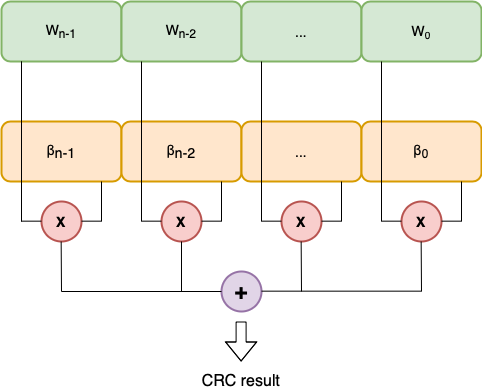
\includegraphics[width=\columnwidth]{figures/PCRC.png}
   \caption{ILLUSTRATION OF  PARALLEL CRC ALGORITHM OVER CHUNK OF M BITS}
   \label{fig:PCRC}
\end{figure}

In this section we present our \textbf{“Parallel Cyclic Redundancy Check” (PCRC) 
algorithm} that performs CRC computation for any length of message in parallel. 

For a given message with any length, we first chunk the message into blocks, 
each of which has a fixed size equal to the degree of the generator polynomial. 
Then we perform CRC computation among the chunked blocks in parallel using 
Galois Field Multiplication and Accumulation (GFMAC).

The message is seen as divided in M bit size chunk and the following is its 
polynomial representation:
\[
   A(x)=W_{n-1}(x)x^{(n-1)M}+\dots{}+W_{1}(x)x^{M}+W_{0}(x)
\]
Where each $W_{i}(x)$ polynomial is a chunk of the message. From this equation 
and the CRC definition, we can compute the CRC for the chunked message by:
\[
   CRC[A(x)]=W_{n-1}x^{nM}modG(x)+\dots{}+W_{0}x^{M}modG(x)
\]
Furthermore, from the Galois Field operations lemma, we obtain that:
\[
\begin{split}
W_{i}(x)x^{(i+1)M}modG(x) = & (W_{i}(x)modG(x) \\& x^{(i+1)M}modG(x))modG(x)
\end{split}
\]
The degree of the polynomial $W_{i}(x)$ for each chunk is $M-1$, therefore it 
is less than $M$, it means that $W_{i}(x)modG(x)=W_{i}(x)$. On the other hand 
the beta coefficients are defined as 
$\beta{}_{i}=x^{(i+1)*M}modG(x)$ for $i=0,1,\dots{},n-1$. Therefore we have:
\[
   CRC[A(x)]=W_{n-1}\otimes{}\beta{}_{n-1}\oplus{}\dots{}
   \oplus{}W_{0}\otimes{}\beta{}_{0}
\]

Note that the operations $\otimes{}$, $\oplus{}$ in the above equation is 
Galois Field multiplication, addition over $GF(2^{M})$, respectively.

The following algorithm is illustrated in Figure \ref{fig:PCRC}.
\begin{enumerate}
   \item Load $N$-bit message in the chunked form of ($W_{n-1},W_{n-2},W_{0}$)
   where each chunk is M bits. \\
   (Note: $N=nM$).

   \item Initially setup the generator polynomial $G(x)$ and its degree $M$. In
   the same time, pre-compute the beta factors 
   ($\beta{}_{n-1},\beta{}_{n-2},\beta{}_{0}$) which depend only on the 
   polynomial and its degree.

   \item Perform $n$-pair Galois field multiplications in
   parallel and then XOR the products. \textbf{This generates the CRC results}.
\end{enumerate}

To compute the beta factors, we have:
\begin{gather*}
   \beta{}_{0}=x^{M}modG(x)=[g_{m-1},\dots,g_{0}] \\
   \beta{}_{1}=x^{2M}modG(x)=\beta{}_{0}\otimes{}\beta{}_{0}=\beta{}_{0}^{2} \\
   \dots{} \\
   \beta{}_{n-1}=x^{nM}modG(x)=\beta{}_{0}^{n}
\end{gather*}
Note that beta factors ($\beta{}_{n-1},\beta{}_{n-2},\beta{}_{0}$) 
do not depend on the incoming message but only on the generator polynomial. 
Since the polynomial is static, this should be pre-computed once and used 
repeatedly in the CRC calculation.

A \textbf{simple pseudocode to generate the beta array could be}:
\begin{verbatim}
for i in range(0 : N)
{
   shift_buffer = 1 << (M * (i + 1));
   beta[i]] = mod2(shift_buffer, 
                   generator_poly);
} 
\end{verbatim}

Each thread is executed over a $M$ bit size chunk of the original message and 
performs the following operations:
\begin{verbatim}
// Get the data of this thread.
W_i = orginal_message[global_index];
beta_i = beta[global_index];

// Perform binary modulo 2 multiplication.
mul = mod2_mul(W_i, beta_i);

// Perform binary modulo 2 reminder.
mod = mod2_mod(mul, generator_poly);

// Copy in shared memory.
shared_memory[threadX] = mod;
sync();

// XOR all data in shared memory.
return xored(shared_memory);
\end{verbatim}

The last operation, that performs the Galois Field addition, xoring all the 
results of the Galois Field multiplication calculated from each thread, 
has been done in 2 ways:
\begin{enumerate}
   \item The standard implementation takes the first thread, stop all the 
   other and performs the XOR operation on all shared memory. This solution 
   has a problem of divergence because one thread is in execution while the 
   other has nothing to do.
   \item The reduction implementation takes the first half of all thread and 
   performs iteratively the XOR operation between a pair of values in shared 
   memory. In this way the workload is more spread across all threads and 
   there is less divergence.
\end{enumerate}

Finally, since the thread execution is done in blocks, the result of the 
device execution will be an array of partial results. Each value of the 
array of partial results will be the xored value of all the Galois Field 
multiplication of the message chunk of that specific thread block. 
Therefore the host has to perform the XOR operation over the array of partial 
results to find the right CRC code. The Figure \ref{fig:PCRC-Reduction} 
shows how the CRC result is obtained by the xoring computation over 
the thread blocks.

\begin{figure}[bt]
\centering
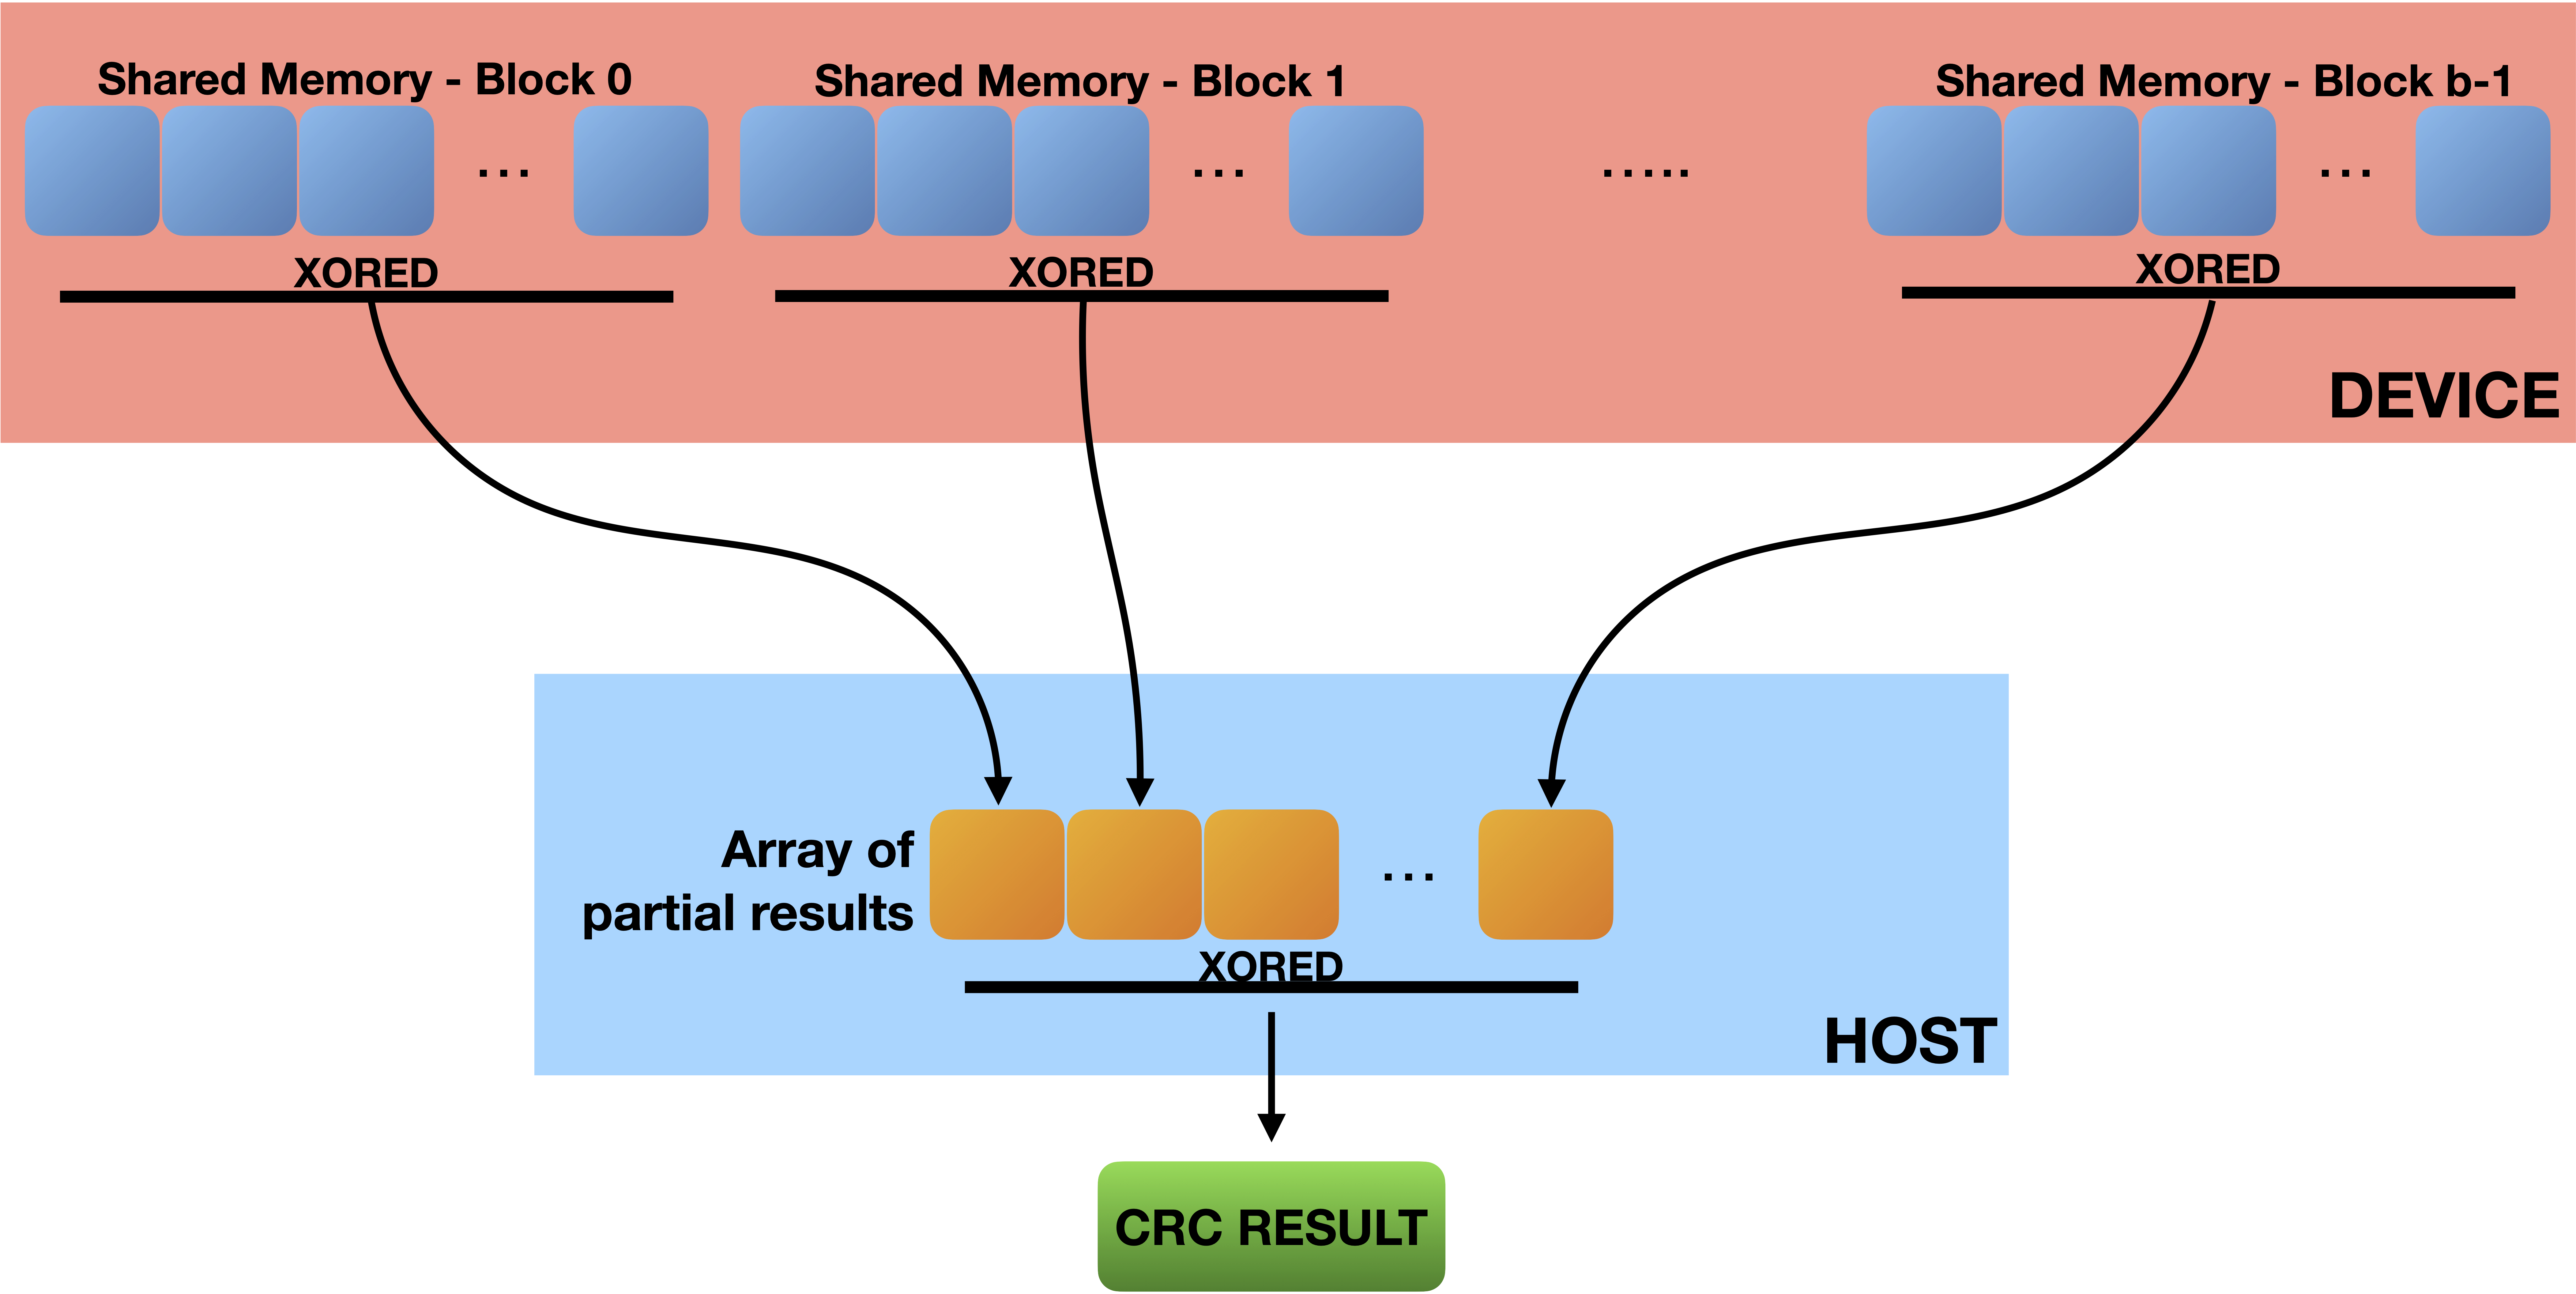
\includegraphics[width=\columnwidth]{figures/PCRC-reduction.png}
\caption{XOR OPERATIONS PERFORM BY DEVICE IN RELATION WITH THE ONE PERFORM BY HOST}
\label{fig:PCRC-reduction}
\end{figure}
\section{Performance analysis}
Theoretically this level of performance is hundreds of 
times faster than bitwise CRC algorithm or tens of times faster than 
bytewise parallel CRC algorithm.

With our software implementation we have achieved the following results:

\subsection{$N=2^{16}$. $BlockSize=64$. $StreamDim=4$. $SegSize=N/StreamDim$}
\begin{footnotesize}
\begin{tabular}{l|l|l|l|l|r|r|r|r|r|r||c|c|}
\toprule
\textbf{Test PCRC 64 blocksize} & \textbf{Speedup} \\
\midrule
PCRC8                                           &	34.71340 \\
PCRC8 with reduction                            &	37.40804 \\
PCRC8 with task parallelism                     &	27.86828 \\
PCRC8 bytewise comparison                       &	2.58712  \\
PCRC8 bytewise comparison with reduction:       &	2.61057  \\
PCRC8 bytewise comparison with task parallelism &	1.93434  \\
PCRC16                                           &	34.98040 \\
PCRC16 with reduction                            &	40.59672 \\
PCRC16 with task parallelism                     &	26.11727 \\
PCRC16 bytewise comparison                       &	3.44060  \\
PCRC16 bytewise comparison with reduction:       &	3.85280  \\
PCRC16 bytewise comparison with task parallelism &	1.51222  \\
PCRC32                                           &	20.23205 \\
PCRC32 with reduction                            &	20.01593 \\
PCRC32 with task parallelism                     &	8.46386  \\
PCRC32 bytewise comparison                       &	1.78715  \\
PCRC32 bytewise comparison with reduction:       &	1.86166  \\
PCRC32 bytewise comparison with task parallelism &	0.71914  \\
\bottomrule
\end{tabular}
\end{footnotesize}

\subsection{$N=2^{16}$. $BlockSize=128$. $StreamDim=4$. $SegSize=N/StreamDim$}
\begin{footnotesize}
\begin{tabular}{l|l|l|l|l|r|r|r|r|r|r||c|c|}
\toprule
\textbf{Test PCRC 128 blocksize} & \textbf{Speedup} \\
\midrule
PCRC8                                           &	34.63720 \\
PCRC8 with reduction                            &	37.41059 \\
PCRC8 with task parallelism                     &	28.19650 \\
PCRC8 bytewise comparison                       &	2.24552  \\
PCRC8 bytewise comparison with reduction:       &	2.70207  \\
PCRC8 bytewise comparison with task parallelism &	2.02773  \\
PCRC16                                           &	34.14637 \\
PCRC16 with reduction                            &	40.48397 \\
PCRC16 with task parallelism                     &	25.37525 \\
PCRC16 bytewise comparison                       &	3.57066  \\
PCRC16 bytewise comparison with reduction:       &	3.60613  \\
PCRC16 bytewise comparison with task parallelism &	1.49754  \\
PCRC32                                           &	20.41607 \\
PCRC32 with reduction                            &	21.54121 \\
PCRC32 with task parallelism                     &	8.51250  \\
PCRC32 bytewise comparison                       &	1.89645  \\
PCRC32 bytewise comparison with reduction:       &	1.85455  \\
PCRC32 bytewise comparison with task parallelism &	0.79350  \\
\bottomrule
\end{tabular}
\end{footnotesize}

\subsection{$N=2^{16}$. $BlockSize=256$. $StreamDim=4$. $SegSize=N/StreamDim$}
\begin{footnotesize}
\begin{tabular}{l|l|l|l|l|r|r|r|r|r|r||c|c|}
\toprule
\textbf{Test PCRC 256 blocksize} & \textbf{Speedup} \\
\midrule
PCRC8                                           &	35.11670 \\
PCRC8 with reduction                            &	37.36065 \\
PCRC8 with task parallelism                     &	29.85230 \\
PCRC8 bytewise comparison                       &	2.66612  \\
PCRC8 bytewise comparison with reduction:       &	2.71714  \\
PCRC8 bytewise comparison with task parallelism &	2.00425  \\
PCRC16                                           &	33.09628 \\
PCRC16 with reduction                            &	39.25975 \\
PCRC16 with task parallelism                     &	27.58368 \\
PCRC16 bytewise comparison                       &	3.53824  \\
PCRC16 bytewise comparison with reduction:       &	3.66416  \\
PCRC16 bytewise comparison with task parallelism &	1.54122  \\
PCRC32                                           &	20.29566 \\
PCRC32 with reduction                            &	21.39834 \\
PCRC32 with task parallelism                     &	7.98474  \\
PCRC32 bytewise comparison                       &	1.75776  \\
PCRC32 bytewise comparison with reduction:       &	1.80291  \\
PCRC32 bytewise comparison with task parallelism &	0.68456  \\
\bottomrule
\end{tabular}
\end{footnotesize}

\subsection{$N=2^{16}$. $BlockSize=128$. $StreamDim=2$. $SegSize=N/StreamDim$}
\begin{footnotesize}
\begin{tabular}{l|l|l|l|l|r|r|r|r|r|r||c|c|}
\toprule
\textbf{Test PCRC 128 blocksize} & \textbf{Speedup} \\
\midrule
PCRC8                                           &	21.32339 \\
PCRC8 with reduction                            &	39.41265 \\
PCRC8 with task parallelism                     &	32.97171 \\
PCRC8 bytewise comparison                       &	2.70535  \\
PCRC8 bytewise comparison with reduction:       &	2.64768  \\
PCRC8 bytewise comparison with task parallelism &	2.48787  \\
PCRC16                                           &	33.66302 \\
PCRC16 with reduction                            &	38.77745 \\
PCRC16 with task parallelism                     &	30.44083 \\
PCRC16 bytewise comparison                       &	3.46636  \\
PCRC16 bytewise comparison with reduction:       &	3.59283  \\
PCRC16 bytewise comparison with task parallelism &	2.80089  \\
PCRC32                                           &	20.42403 \\
PCRC32 with reduction                            &	21.38471 \\
PCRC32 with task parallelism                     &	7.35099  \\
PCRC32 bytewise comparison                       &	1.87434  \\
PCRC32 bytewise comparison with reduction:       &	1.86528  \\
PCRC32 bytewise comparison with task parallelism &	0.72902  \\
\bottomrule
\end{tabular}
\end{footnotesize}

\subsection{$N=2^{16}$. $BlockSize=128$. $StreamDim=8$. $SegSize=N/StreamDim$}
\begin{footnotesize}
\begin{tabular}{l|l|l|l|l|r|r|r|r|r|r||c|c|}
\toprule
\textbf{Test PCRC 128 blocksize} & \textbf{Speedup} \\
\midrule
PCRC8                                           &	35.05756 \\
PCRC8 with reduction                            &	38.59024 \\
PCRC8 with task parallelism                     &	11.97966 \\
PCRC8 bytewise comparison                       &	2.65855  \\
PCRC8 bytewise comparison with reduction:       &	2.73349  \\
PCRC8 bytewise comparison with task parallelism &	1.20074  \\
PCRC16                                           &	34.06469 \\
PCRC16 with reduction                            &	38.96202 \\
PCRC16 with task parallelism                     &	11.68695 \\
PCRC16 bytewise comparison                       &	3.87572  \\
PCRC16 bytewise comparison with reduction:       &	3.22093  \\
PCRC16 bytewise comparison with task parallelism &	1.58960  \\
PCRC32                                           &	20.83102 \\
PCRC32 with reduction                            &	22.14467 \\
PCRC32 with task parallelism                     &	6.38649  \\
PCRC32 bytewise comparison                       &	1.94807  \\
PCRC32 bytewise comparison with reduction:       &	1.91344  \\
PCRC32 bytewise comparison with task parallelism &	0.65893  \\
\bottomrule
\end{tabular}
\end{footnotesize}

\subsection{$N=2^{16}$. $BlockSize=128$. $StreamDim=4$. $SegSize=N/8$}
\begin{footnotesize}
\begin{tabular}{l|l|l|l|l|r|r|r|r|r|r||c|c|}
\toprule
\textbf{Test PCRC 128 blocksize} & \textbf{Speedup} \\
\midrule
PCRC8                                           &	35.41841 \\
PCRC8 with reduction                            &	40.88182 \\
PCRC8 with task parallelism                     &	17.13281 \\
PCRC8 bytewise comparison                       &	2.40438  \\
PCRC8 bytewise comparison with reduction:       &	2.97784  \\
PCRC8 bytewise comparison with task parallelism &	0.47928  \\
PCRC16                                           &	34.66451 \\
PCRC16 with reduction                            &	42.29803 \\
PCRC16 with task parallelism                     &	16.70620 \\
PCRC16 bytewise comparison                       &	4.04358  \\
PCRC16 bytewise comparison with reduction:       &	3.76574  \\
PCRC16 bytewise comparison with task parallelism &	1.51226  \\
PCRC32                                           &	21.27053 \\
PCRC32 with reduction                            &	21.97304 \\
PCRC32 with task parallelism                     &	7.47568  \\
PCRC32 bytewise comparison                       &	1.92987  \\
PCRC32 bytewise comparison with reduction:       &	1.90569  \\
PCRC32 bytewise comparison with task parallelism &	0.52763  \\
\bottomrule
\end{tabular}
\end{footnotesize}

\subsection{NVIDIA Nsight Graphics}
\textbf{NVIDIA Nsight Graphics} is a low overhead performance analysis tool 
designed to provide insights developers need to optimize their software. 
Unbiased activity data is visualized within the tool to help users investigate 
bottlenecks, avoid inferring false-positives, and pursue optimizations with 
higher probability of performance gains. Users will be able to identify issues, 
such as GPU starvation, unnecessary GPU synchronization, insufficient CPU 
parallelizing, and even unexpectedly expensive algorithms across the CPUs and 
GPUs of their target platform.

The Figure \ref{fig:NSG-PCRC8} shows the standard algorithm profiling where 
you can see on the left the kernel execution rates compared to memory transfer.

In the Figure \ref{fig:NSG-PCRC8-reduction} you can see how this time kernel 
execution prevails because there is less divergence. 

With the Figure \ref{fig:NSG-PCRC8-task-parallelism-1} and 
\ref{fig:NSG-PCRC8-task-parallelism-2} you can see that 
execution is split over multiple streams and that in some cases, 
in the timeline, kernel execution and memory transfer occurs in parallel.


\begin{figure*}[bt]
\centering
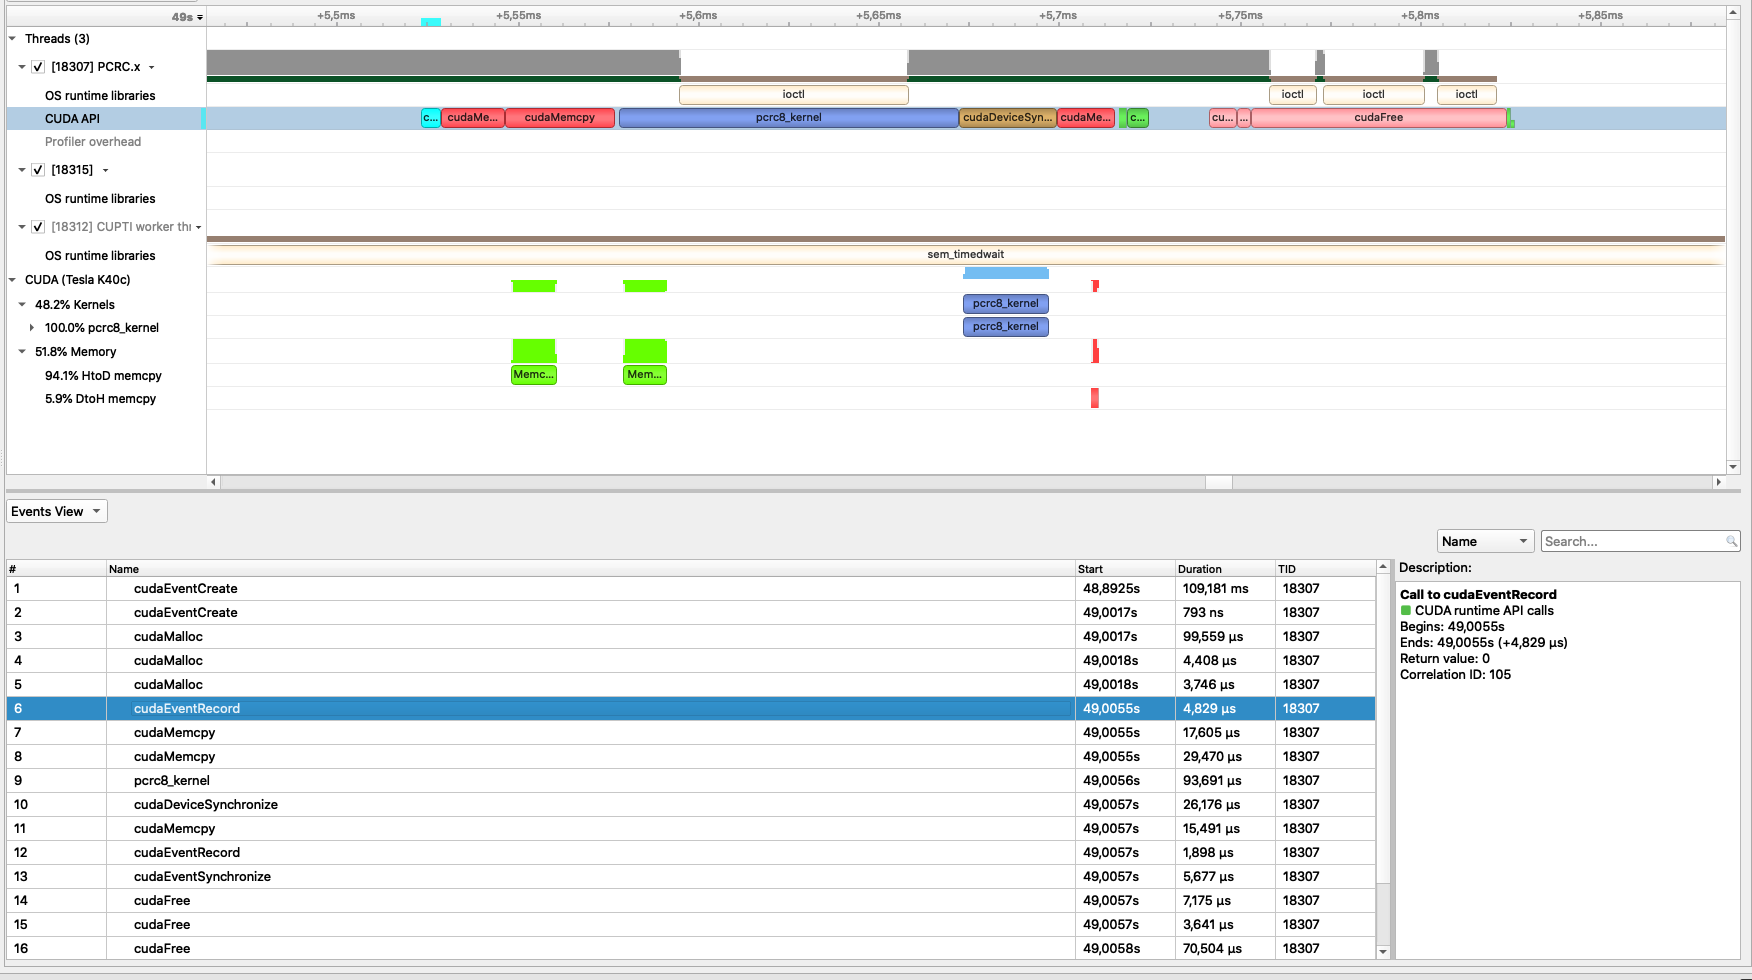
\includegraphics[width=\textwidth]{figures/NSG-PCRC8.png}
\caption{NVIDIA NSIGHT GRAPHICS PCRC8}
\label{fig:NSG-PCRC8}
\end{figure*}

\begin{figure*}[bt]
\centering
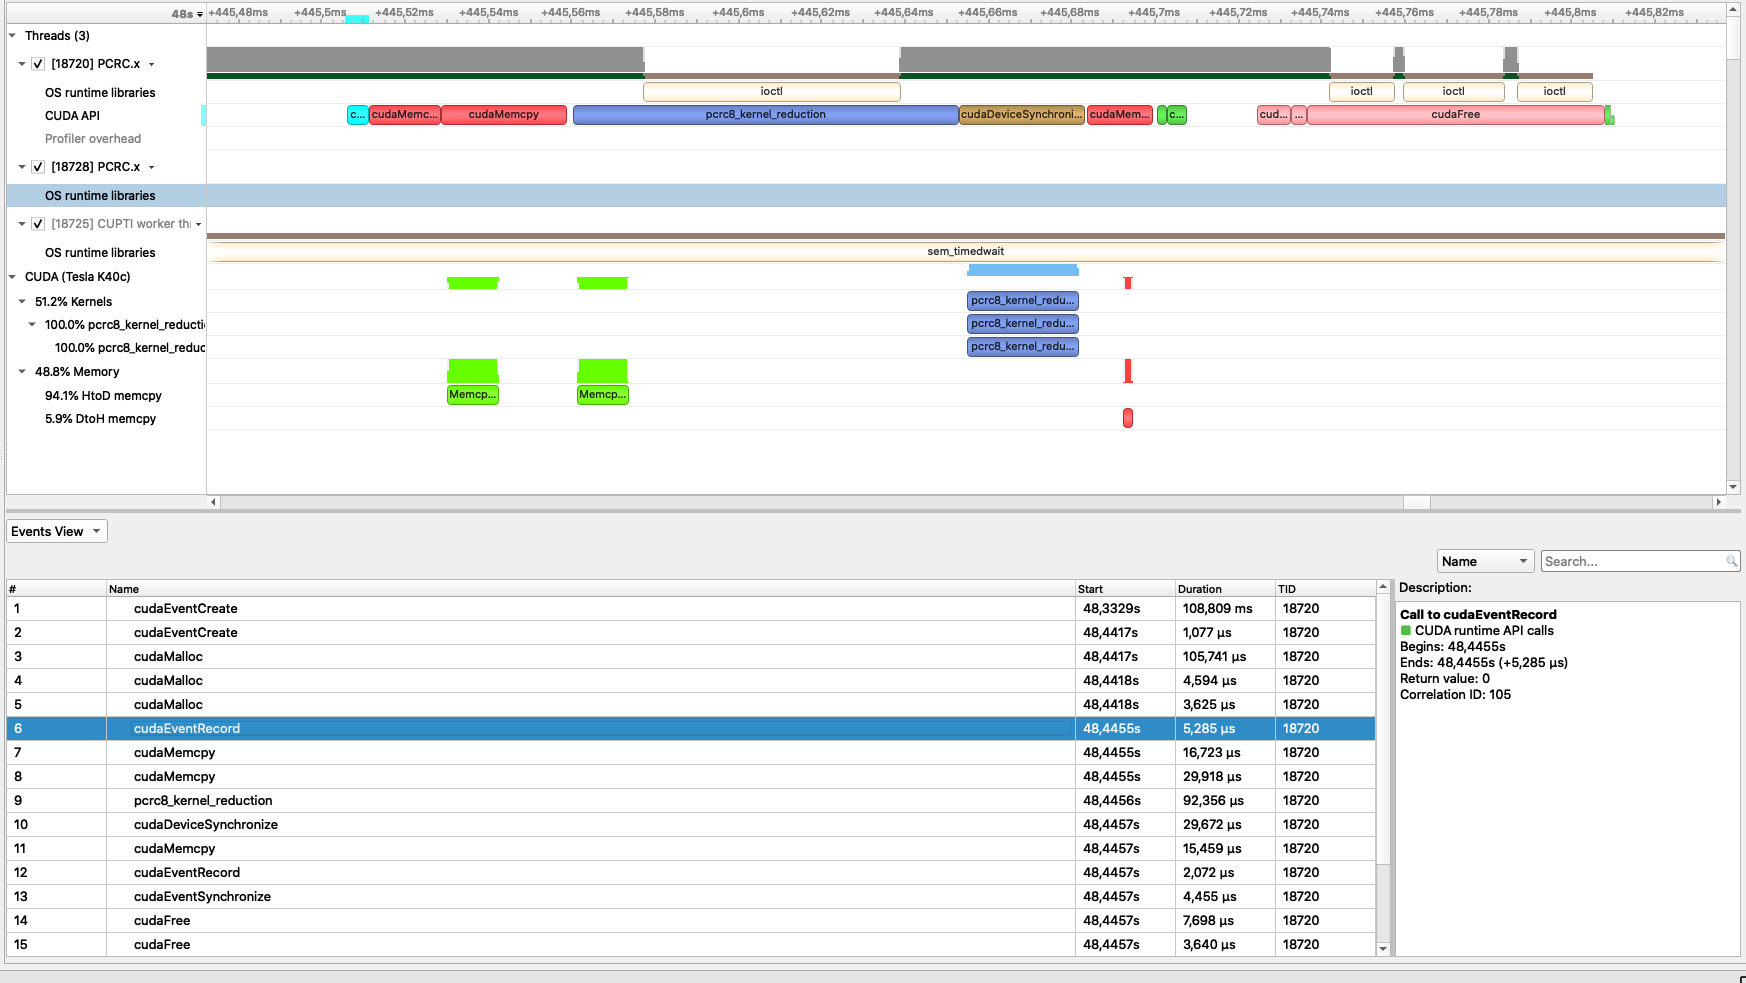
\includegraphics[width=\textwidth]{figures/NSG-PCRC8-reduction.png}
\caption{NVIDIA NSIGHT GRAPHICS PCRC8 REDUCTION}
\label{fig:NSG-PCRC8-reduction}
\end{figure*}

\begin{figure*}[bt]
\centering
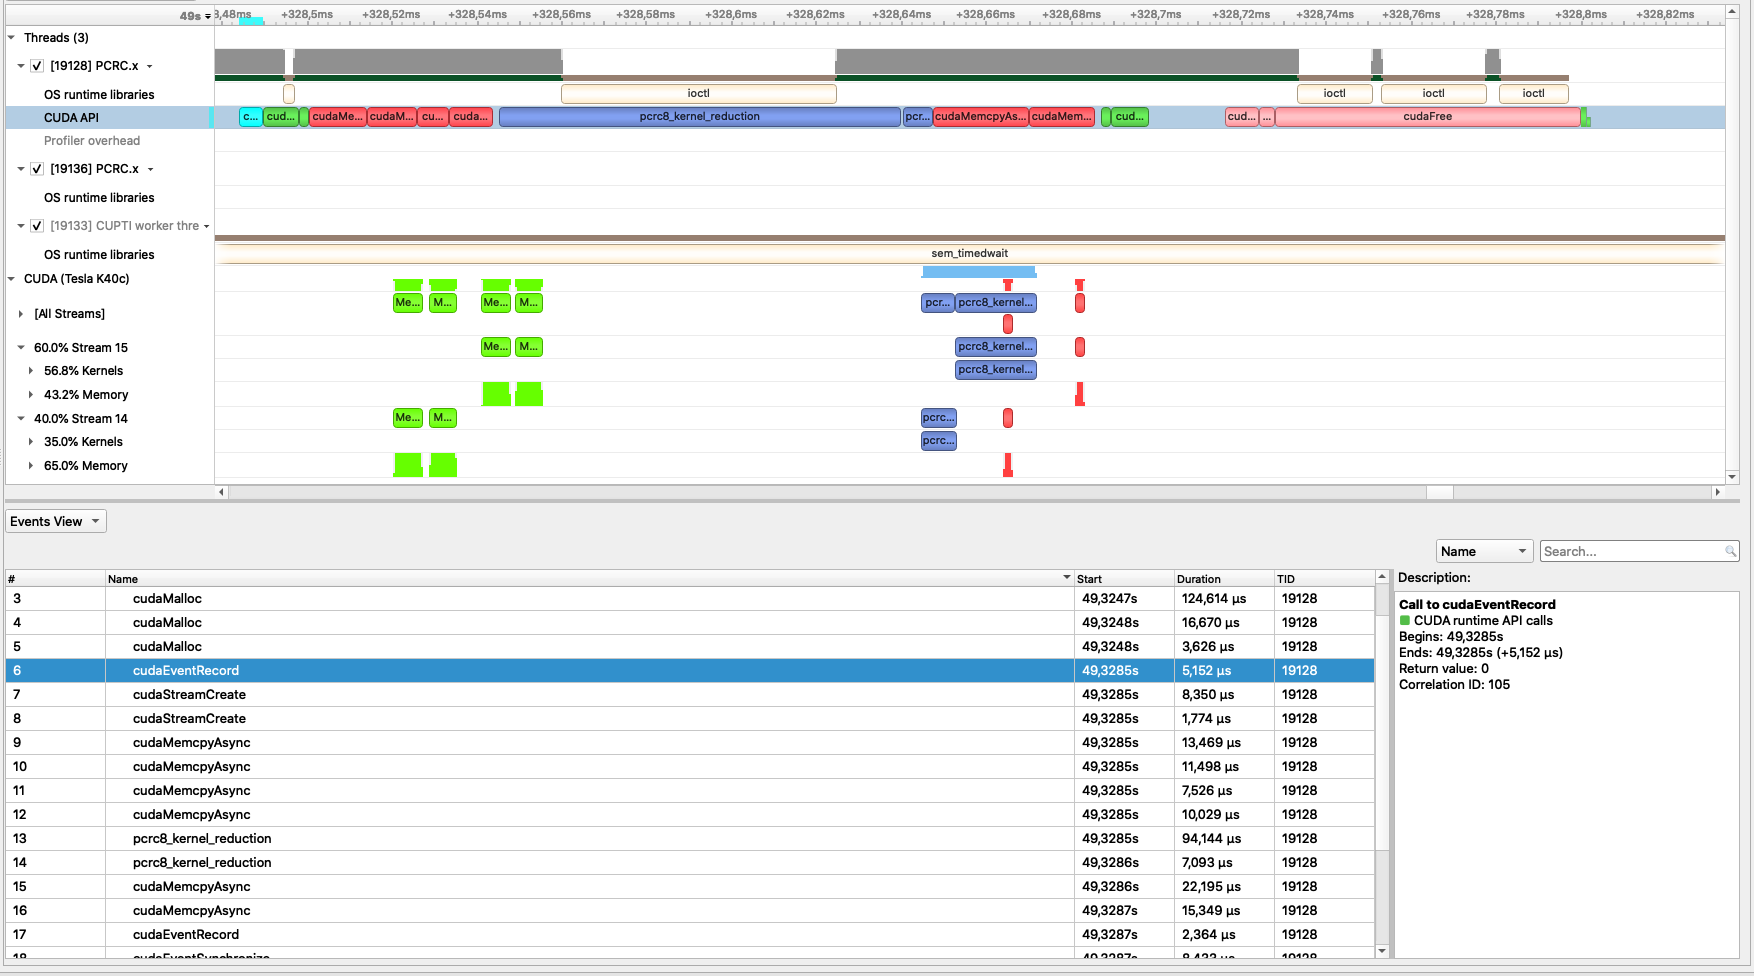
\includegraphics[width=\textwidth]{figures/NSG-PCRC8-task-parallelism-1.png}
\caption{NVIDIA NSIGHT GRAPHICS PCRC8 TASK PARALLELISM - CASE 1}
\label{fig:NSG-PCRC8-task-parallelism-1}
\end{figure*}

\begin{figure*}[bt]
\centering
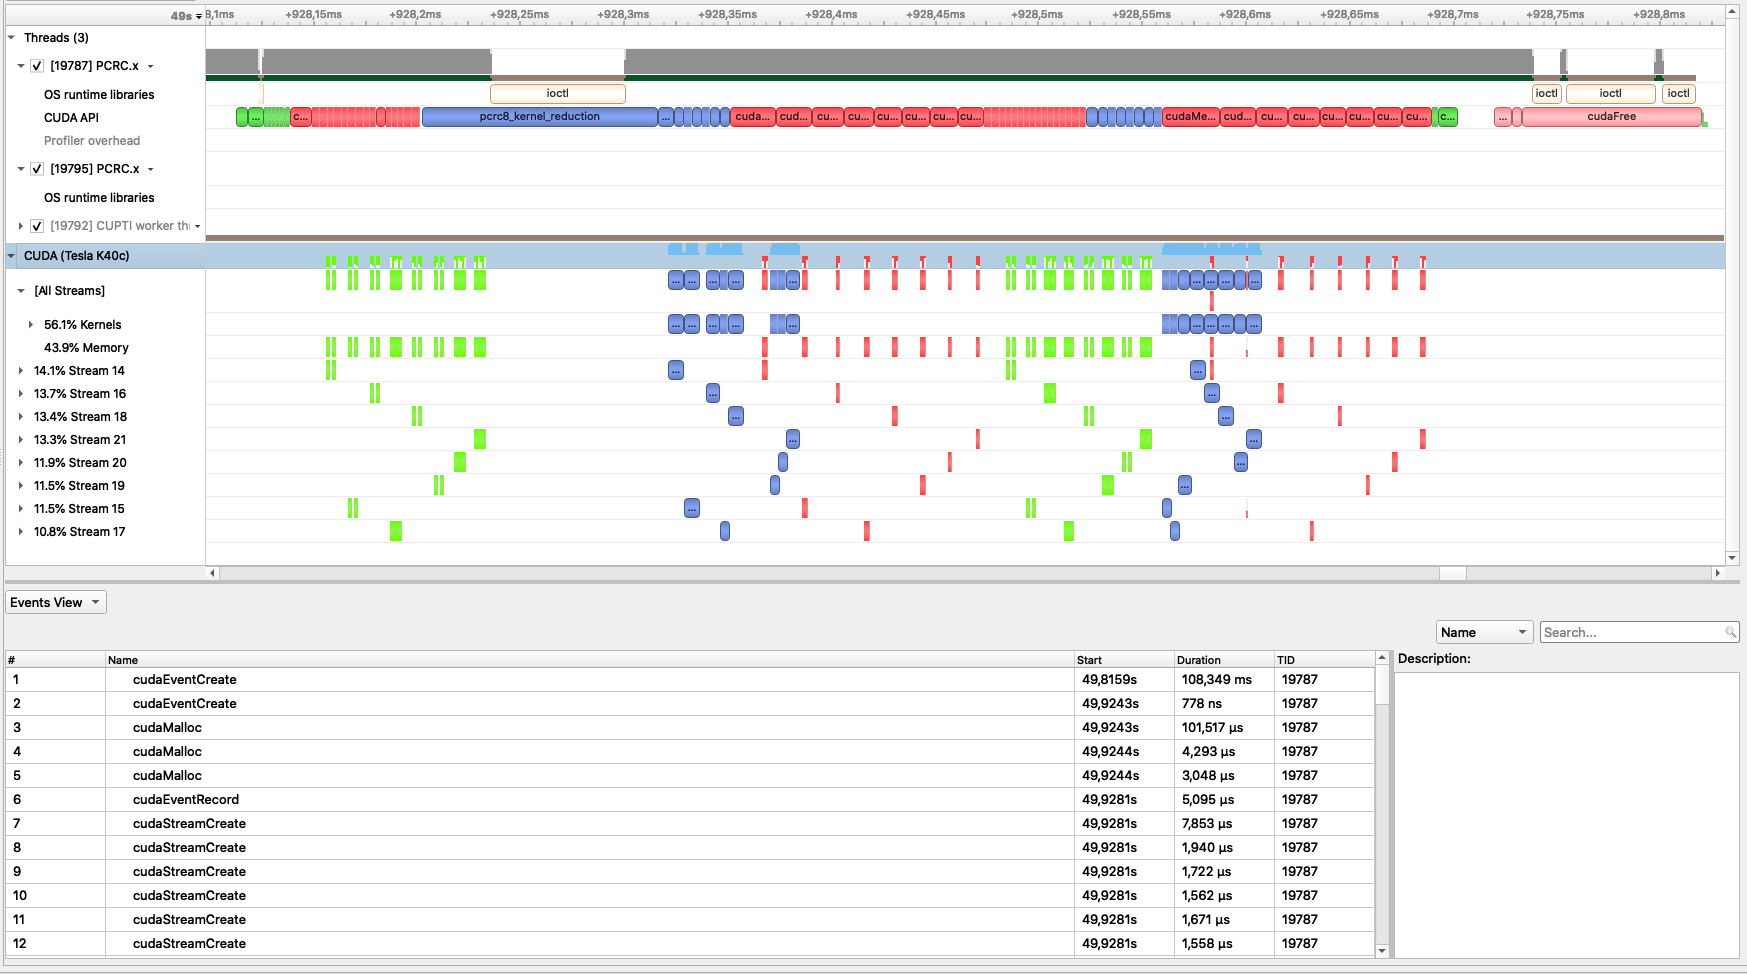
\includegraphics[width=\textwidth]{figures/NSG-PCRC8-task-parallelism-2.png}
\caption{NVIDIA NSIGHT GRAPHICS PCRC8 TASK PARALLELISM - CASE 2}
\label{fig:NSG-PCRC8-task-parallelism-2}
\end{figure*}

\section{Conclusions}
This paper shows a systematic method to calculate CRC in parallel using the 
Galois Field property. The method can be easily expanded to all feasible $r$ 
parallel-input bits for fast CRC calculation without added complexity in the 
developing process or practical limitation like the size of lookup tables 
needed in other approaches.

The implementation with tasks parallelism does not give better performance 
because the overhead of the technique is not positively compensated on the 
improvement that leads to performance. So the best result with parallelism 
tasks is obtained for $StreamDim=4$ and $SegSize=N/StreamDim$. 

In general the best performances are with $BlockSize=128$, while in the case of 
parallelism tasks the best performances are with $StreamDim=2$ and 
$SegSize=N/StreamDim$ using the reduction algorithm that reduces the divergence 
of the threads, which on average increases the performance compared to the 
standard solution of some speedup units.

\textbf{From these results we can say that the PCRC speedup is more $+2.5$}.
\end{document}